\documentclass[class=report,crop=false, 12pt]{standalone}
\usepackage[screen,nosolutions]{../scratch}

%\usepackage[print]{../scratch}

\begin{document}

\titre[S]{Plusieurs lutins}
%===============================

\insertvideo{c49ESfUtsCQ}{Plusieurs lutins -- Activité 1}

\insertvideo{FkwNPsQIGzQ}{Plusieurs lutins -- Activité 2}

\insertvideo{tKNwYbBzYUU}{Plusieurs lutins -- Activité 3}

\bigskip
\bigskip

\begin{activite}


Programme quatre chats qui courent les uns après les autres :

\begin{center}
  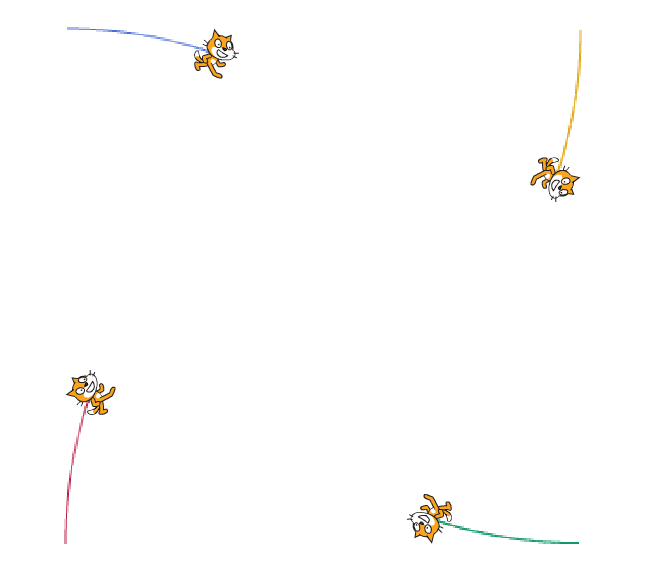
\includegraphics[scale=\scaleecran]{ecran-08-ex1} 
\end{center}

\begin{itemize}
  \item le chat 1 court après le chat 2,
  \item le chat 2 court après le chat 3,
  \item le chat 3 court après le chat 4,
  \item le chat 4 court après le chat 1.
\end{itemize}

\bigskip

Voici les positions et orientations de départ :
\myfigure{0.9}{
\tikzinput{carre-chat}
}  

\bigskip
\textbf{Plusieurs lutins.}

Avec Scratch, tu peux contrôler plusieurs lutins en même temps.
Chaque lutin aura ses propres instructions.
Pour définir un nouveau lutin, clique sur l'icône \og nouveau lutin \fg{}
ou bien clique le bouton droit de la souris sur un lutin existant, puis sur \og dupliquer \fg{}.


\bigskip


\textbf{Blocs utiles.}

\begin{center}
  
\includegraphics[scale=\scalebloc]{bloc-08-ex1} 
\end{center} 


  
\end{activite}




\begin{activite}

Programme un petit jeu de calcul mental avec un chat et trois souris.
\begin{itemize}
  \item Le chat demande le résultat d'une multiplication.
  \item La souris 1 affiche le bon résultat.
  \item Les souris 2 et 3 affichent des résultats faux.
  \item Le chat doit avancer en suivant le pointeur de la souris de l'ordinateur jusqu'à toucher la souris qui affiche le bon résultat.
\end{itemize}

\begin{center}
  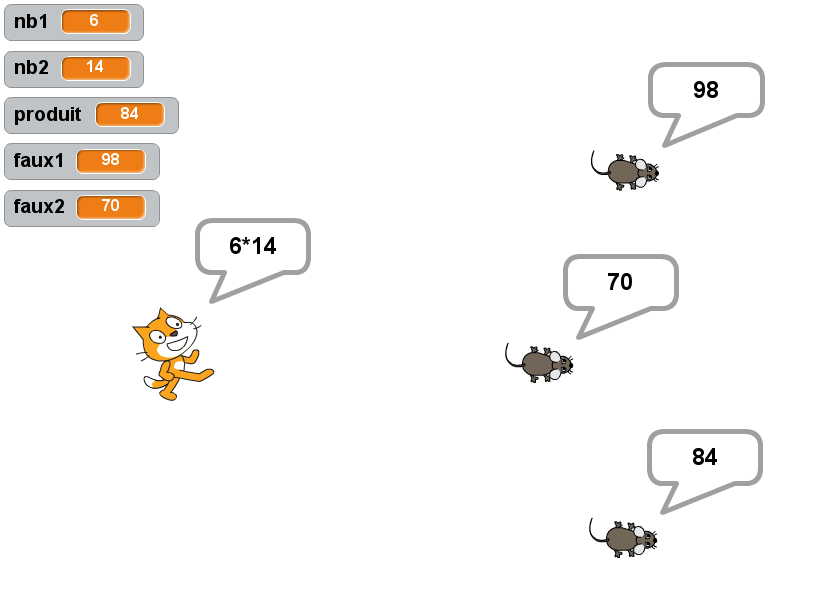
\includegraphics[scale=\scaleecran]{ecran-08-ex2} 
\end{center}

\bigskip
Voici comment structurer ton programme :

\bigskip

\begin{itemize}
  \item \textbf{Initialisation.}
  
  Débute par les instructions suivantes, qui peuvent être incluses avec celles du chat.
  \begin{itemize}
    \item Choisis deux nombres \codeinline{nb1} et \codeinline{nb2} au hasard entre $5$ et $15$.
    \item La bonne réponse sera \codeinline{produit} = \codeinline{nb1} $\times$  \codeinline{nb2}.
    \item Deux mauvaises réponses seront proposées par exemple :   
    \codeinline{faux1} = $($\codeinline{nb1} $+1) \times$  \codeinline{nb2} et     
    \codeinline{faux2} = $($\codeinline{nb1} $-1) \times$  \codeinline{nb2}.
        
  \end{itemize}

\bigskip

  \item \textbf{Le chat.}  
  \begin{itemize}
    \item Il démarre de la gauche.
    \item Il affiche l'opération \og \codeinline{nb1} $\times$  \codeinline{nb2} \fg{}.
    \item On répète indéfiniment : s'orienter vers le pointeur de la souris de l'ordinateur et avancer de $3$ pas.
    \item S'il touche la souris 1, c'est gagné !
  \end{itemize}

\bigskip

  \item \textbf{Les souris.}  
  \begin{itemize}
    \item Chaque souris se place au hasard, avec $x$ entre $0$ et $150$ et 
    $y$ entre $-150$ et $150$.
    \item La souris $1$ affiche \codeinline{produit}, les autres souris affichent
    les mauvais résultats \codeinline{faux1} et \codeinline{faux2}.
  \end{itemize}  
\end{itemize}    
   
\end{activite}




\begin{activite}

Programme un canon qui lance une balle. Si la balle touche le chien, c'est gagné !
On peut régler l'orientation du canon par un angle et aussi régler la puissance du lancer.

\begin{center}
  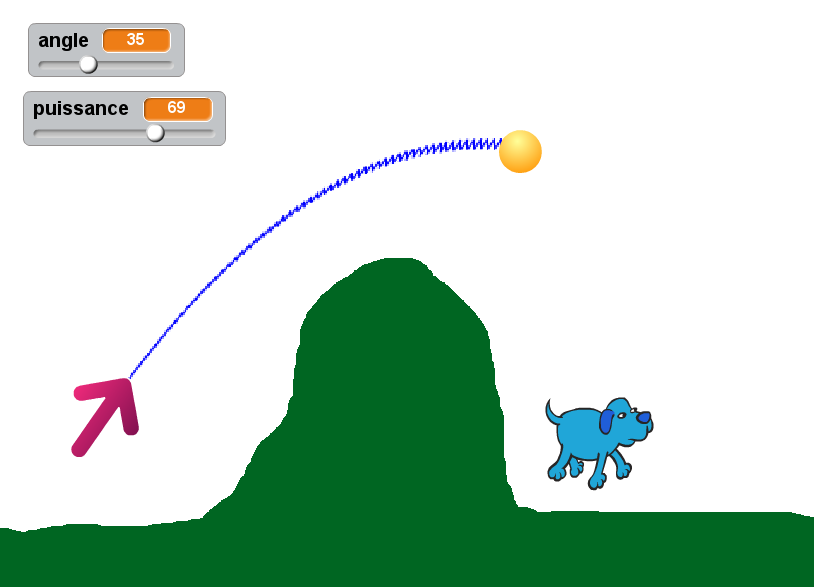
\includegraphics[scale=\scaleecran]{ecran-08-ex3} 
\end{center}



\textbf{Le canon.}

\begin{itemize}
  \item Définis une variable \codeinline{angle}.
  \item Répète indéfiniment : s'orienter à \codeinline{angle}.
  \item Une fois le programme lancé, tu peux régler l'angle à l'aide d'un curseur (affiche la variable \codeinline{angle} et double clique sur cet affichage, jusqu'à obtenir le potentiomètre).
\end{itemize}

\bigskip

\textbf{L'arrière-plan et le chien}
\begin{itemize}
  \item Dessine un arrière-plan coloré (ici vert), avec une montagne au milieu afin d'éviter un tir direct.
  \item Place un chien à droite de la montagne. Pour compliquer la mission, le chien peut être en mouvement de gauche à droite.
\end{itemize}

\bigskip
\textbf{La balle : tir parabolique.}

C'est la partie la plus délicate. Une fois la balle lancée, elle suit une trajectoire en forme de parabole. Le principe est expliqué plus loin.

Dans la pratique :
\begin{itemize}
  \item Définir une variable \codeinline{puissance} (réglable comme pour \codeinline{angle} ci-dessus).

  \item Définir une variable \codeinline{descente} et l'initialiser à $0$.
  
  \item Orienter la balle à \codeinline{angle}.
  
  \item Répéter :
  \begin{itemize}
    \item avancer de $0.1 \times$\codeinline{puissance},
    
    \item ajouter $-0.1$ à \codeinline{descente},
    
    \item ajouter \codeinline{descente} à $y$.
    
  \end{itemize}
\end{itemize}


\bigskip
\textbf{La balle : gagné ou perdu ?}

\begin{itemize}
  \item Si la balle touche la couleur verte ou si la balle touche le bord de l'écran : c'est perdu.
  \item Si la balle touche le chien : c'est gagné !
\end{itemize}


\bigskip

Voici le principe du tracé du tir parabolique : 
\begin{itemize}
  \item La trajectoire est formée de petits segments.
  \item Chaque segment s'obtient en suivant deux vecteurs (des \og flèches \fg{}).
  \item Le premier vecteur est déterminé par l'angle et la puissance : il reste tout le temps le même.
  \item Le second vecteur est un vecteur vertical dirigé vers le bas. Ce vecteur va être de plus en plus grand (c'est la variable \codeinline{descente}).
  \item Le segment à tracer part au début du premier vecteur et arrive à la fin du second.
  \item On recommence, mais avec un vecteur vertical un peu plus grand.
\end{itemize}  

\myfigure{1.1}{
\tikzinput{parabole1}
\quad
\tikzinput{parabole2}
\quad
\tikzinput{parabole3}
\quad
}  


\myfigure{0.5}{
\tikzinput{parabole4}
}  

\end{activite}


\ifx \displaysolutions \myzero
\else
\begin{code}
\onesolution{Plusieurs lutins}{Activité 1}{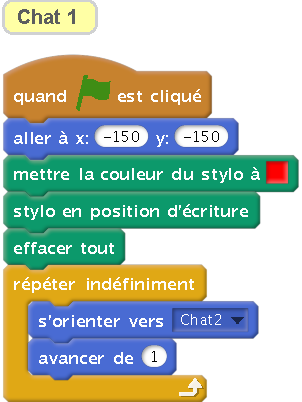
\includegraphics[scale=\scalesolution]{code-08-ex1}}
\onesolution{Plusieurs lutins}{Activité 2}{
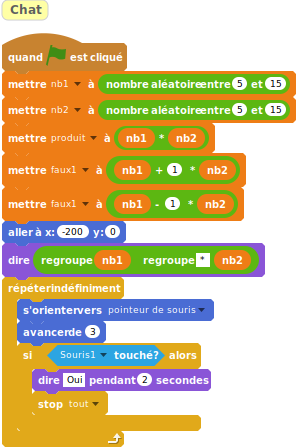
\includegraphics[scale=\scalesolution]{code-08-ex2a}
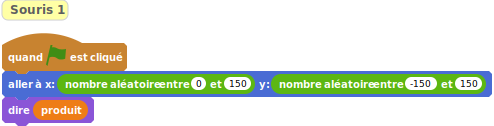
\includegraphics[scale=\scalesolution,scale=0.7]{code-08-ex2b} 
}
\onesolution{Plusieurs lutins}{Activité 3}{
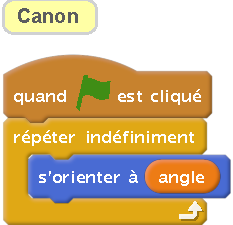
\includegraphics[scale=\scalesolution]{code-08-ex3a}
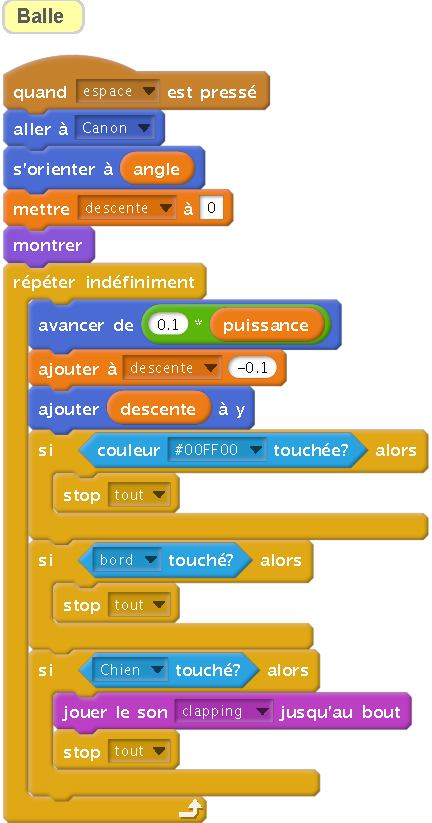
\includegraphics[scale=\scalesolution]{code-08-ex3b}
} 

\medskip

Cette dernière activité s'inspire de \href{https://scratch.mit.edu/projects/33928/}{https://scratch.mit.edu/projects/33928/} par Dave911.
\end{code}
\fi

\end{document}

